\documentclass{ximera}

\input{../preamble.tex}


\title[Dig-In:]{The gradient}

\begin{document}
\begin{abstract}
We introduce the gradient vector. 
\end{abstract}
\maketitle

The gradient is a useful tool in vector calculus. In some sense, it
has the role that the derivative has in single-variable calculus.
Let's state the definition:

\begin{definition}
  Let $F:\R^n\to \R$ be a differentiable function, the \dfn{gradient}
  \[
  \grad F = \vector{\pp[F]{x_1},\pp[F]{x_2},\dots,\pp[F]{x_n}}
  \]
  is a vector-valued function of $n$ variables. 
\end{definition}

Try your hand at some casual computations.

\begin{question}
  Let $F(x,y) = \sin(x)\cos(y)$, compute:
  \[
  \grad F(x,y)
  \begin{prompt}
    = \vector{\answer{\cos(x)\cos(y)},\answer{-\sin(x)\sin(y)}}
  \end{prompt}
  \]
  \begin{question}
    Let $\vec{p}= \vector{\pi/3,\pi/3}$. Compute:
    \[
    \grad F(\vec{p})
    \begin{prompt}
      =\vector{\answer{1/4},\answer{-3/4}}
    \end{prompt}
    \]
  \end{question}
\end{question}

And now in three variables.

\begin{question}
  Let $F(x,y) = ze^{-7xy}$, compute:
  \[
  \grad F(x,y)
  \begin{prompt}
    = \vector{\answer{z e^{-7xy}(-7)y},\answer{z e^{-7xy}(-7)x}, \answer{e^{-7xy}}}
  \end{prompt}
  \]
  \begin{question}
    Let $\vec{p}= \vector{1,0,1/7}$. Compute:
    \[
    \grad F(\vec{p})
    \begin{prompt}
      =\vector{\answer{0},\answer{-1},\answer{1}}
    \end{prompt}
    \]
  \end{question}
\end{question}

The gradient can help us understand how a function in a particular
direction.

\begin{definition}
  The \dfn{directional derivative} is computed by
  \[
  D_\vec{\hat{u}}(F) = \grad(F(x,y))\dotp \vec{\hat{u}}
  \]
  where $\vec{\hat{u}}$ is a unit vector.
\end{definition}

The directional derivative tells us how $F$ changes if we move one
direction.  Now that we can compute the gradient, let's see if we can
figure out what it \textbf{means}.

\section{The initial greatest increase}

First recall what it means for a function to be \textit{differentiable}:
\begin{quote}\index{tangent plane}%%BADBAD would like an image
  Given a function $F:\R^3\to\R$ and a vector $\vec{a}$ in the domain
  of $F$, if one can ``zoom in'' on the graph at $(\vec{a}, F(\vec{a}))$
  sufficiently so that it appears to be a plane, then the
  function is \dfn{differentiable}, and that plane is the \dfn{tangent plane}
  to $F$ at the point $(\vec{a},F(\vec{a}))$.
\end{quote}

Now let's imagine what the gradient is telling us about the
plane. First let $\vec{p}=\vector{a,b}$ and set
\[
\vector{m_1,m_2} = \grad F(\vec{p})
\]
Now the tangent plane is given by: 
\[
z = m_1 (x-a) + m_2 (y-b) + F(a,b)
\]
what happens if we leave the point $\vec{p}$ in the direction of
\[
\vector{m_1,m_2} = \grad F(\vec{p})?
\]
Well,
\begin{itemize}
  \item if a component of $\grad F(\vec{p})$ is positive, traveling in
    its direction will ensure that you are ``traveling uphill,''
    meaning you are raising the $z$-value (at least initially).
\item if a component of $\grad F(\vec{p})$ is negative, traveling in its
  (negative) direction will also ensure that you are ``traveling
  uphill,'' meaning you are raising the $z$-value (at least
  initially).
\end{itemize}
From this we see that the components of $\grad F(\vec{p})$ form a
vector that simultaneously points ``most uphill'' in the
$x$-direction, and ``most uphill'' in the $y$-direction. The upshot?
\begin{quote}
  \textbf{The gradient points in the initial direction of the greatest
    increase of the function.}
\end{quote}

You may be wondering, ``Why does the gradient only point in the
`initial' direction of greatest increase?''  It can only be
``initial'' because the reasoning above relies on the fact that we can
be ``zoomed-in'' enough for the surface to look like a plane.
\begin{onlineOnly}
For your viewing pleasure, we have included a graph where you can see
the $x$-component of the gradient and the $y$-component of the
gradient combining to give the initial the direction one should leave
from a point, and find the initial greatest increase in the function.
\begin{sageCell}
f(x,y) = 3*x+4*y
vectorx=arrow3d((0,0,0),(3,0,0),7,color='blue');
vectory=arrow3d((0,0,0),(0,4,0),7,color='blue');
grad=arrow3d((0,0,0),(3,4,0),7,color='red');

plot3d( f, (x,-3,3), (y,-3,3) ) + vectorx + vectory + grad
\end{sageCell}
\end{onlineOnly}
\begin{remark}
  Given a function $F:\R\to\R^3$, the vectors $\grad F(x,y)$ are only
  pointing in two dimensions. Consider
  \[
  z = F(x,y) = 3x+4y.
  \]
  This is an explicit function that can be described as a surface in
  three-dimensional space, yet the gradient vector
  \[
  \grad F = \vector{3, 4}
  \]
  is a vector in $\R^2$, meaning two-dimensional space. Similarly, if
  you are working with a function $F:\R\to\R^n$, this can be described
  as a ``surface'' in $(n+1)$-dimensional space, but the gradient
  vectors
  \[
  \vector{\pp[F]{x_1},\pp[F]{x_2},\dots,\pp[F]{x_n}}
  \]
  are vectors in $n$-dimensional space.
\end{remark}


\begin{example}
  Let
  \[
  F(x,y) = -x^2+2x-y^2+2y+1.
  \]
  Compute and interpret $\grad F(1,1)$.
  \begin{explanation}
    Write with me
    \[
    \grad F(x,y) = \vector{\answer[given]{-2x+2},\answer[given]{-2y+2}}.
    \]
    However, we see $\grad F(1,1) = \vector{\answer[given]{0},\answer[given]{0}}$.  Since there is no
    initial direction of greatest increase, we must be at a local
    maximum for the function. Indeed we are, behold:
    \begin{image}
      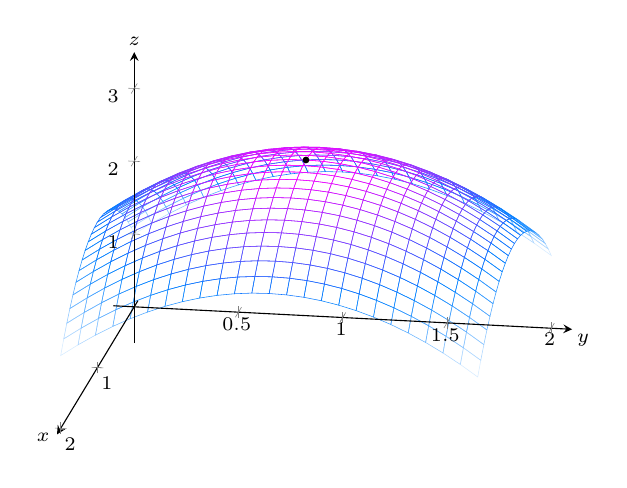
\begin{tikzpicture}
        \begin{axis}%
          [tick label style={font=\scriptsize},axis on top,
	    axis lines=center,
	    view={100}{25},
	    name=myplot,
	    %xtick=\empty,
	    %ytick={5},
	    %ztick={.7,-.7},
	    minor xtick=1,
	    minor ytick=1,
	    ymin=-.1,ymax=2.1,
	    xmin=-.1,xmax=2.1,
	    zmin=-.5, zmax=3.5,
	    every axis x label/.style={at={(axis cs:\pgfkeysvalueof{/pgfplots/xmax},0,0)},xshift=-5pt,yshift=-1pt},
	    xlabel={\scriptsize $x$},
	    every axis y label/.style={at={(axis cs:0,\pgfkeysvalueof{/pgfplots/ymax},0)},xshift=4pt,yshift=-4pt},
	    ylabel={\scriptsize $y$},
	    every axis z label/.style={at={(axis cs:0,0,\pgfkeysvalueof{/pgfplots/zmax})},xshift=0pt,yshift=4pt},
	    zlabel={\scriptsize $z$},
            colormap/cool
	  ]
          
          \addplot3[domain=0:2,,y domain=0:2,
            mesh,samples=25,samples y=25,very thin,z buffer=sort] {-x^2-y^2+2*x+2*y+1};
          \filldraw [black,] (axis cs:1,1,3) circle (1pt);
        \end{axis}
      \end{tikzpicture}
    \end{image}
    Ah! The point $(1,1)$ lies at the top of a paraboloid. In all
    directions, the instantaneous rate of change is $0$.
  \end{explanation}
\end{example}

Stand back. We're going to do some serious calculus now. Just read,
relax and enjoy.

\begin{example}
  Consider the surface given by $F(x,y)= 20-x^2-2y^2$:
  \begin{image}
    \begin{tikzpicture}
      \begin{axis}%
        [tick label style={font=\scriptsize},axis on top,
	  axis lines=center,
	  view={155}{25},
	  name=myplot,
	  %xtick=\empty,
	  %ytick={5},
	  %ztick={.7,-.7},
	  %minor xtick=1,
	  %minor ytick=1,
	  ymin=-1,ymax=5.5,
	  xmin=-1,xmax=5.5,
	  zmin=-1.1, zmax=21,
	  every axis x label/.style={at={(axis cs:\pgfkeysvalueof{/pgfplots/xmax},0,0)},xshift=-5pt,yshift=-1pt},
	  xlabel={\scriptsize $x$},
	  every axis y label/.style={at={(axis cs:0,\pgfkeysvalueof{/pgfplots/ymax},0)},xshift=4pt,yshift=-4pt},
	  ylabel={\scriptsize $y$},
	  every axis z label/.style={at={(axis cs:0,0,\pgfkeysvalueof{/pgfplots/zmax})},xshift=0pt,yshift=4pt},
	  zlabel={\scriptsize $z$},colormap/cool
        ]
        
        %\addplot3[domain=0:180,smooth,y domain=0:360,surf,%fill=white,
        %colormap={mp2}{\colormapplaneone},faceted color=black!40,samples=30,samples y=25,very thin,z buffer=sort] ({cos(x)*1.5*cos(y)},{sin(x)*cos(y)},{sin(y)});
        
        \addplot3[domain=-1:4,y domain=-1:3,mesh,samples y=15,very thin,z buffer=sort,%opacity=.6,
          samples=15,] (x,y,{20-x^2-2*y^2});
        
        \addplot3 [thick, penColor, smooth,domain=1:4,samples=20,samples y=0] ({x},{x^2/4},{20-x^2-0.125*x^4});
        %%        
        \filldraw [black] (axis cs:1,.25,18.875) circle (1pt);
        %\filldraw [black] (axis cs:.5,.25,19.625) circle (1pt);
        %
        %\filldraw [black] (axis cs:.5,.5,19.25) circle (1pt);
        
        
        %\addplot3 [thick,{\colorone}, smooth,domain=-3:3,samples=20,samples y=0] ({x},{2},{x^2+8});
        %
        %\addplot3 [thick,{\colorone}, smooth,domain=-30:170,samples=60,samples y=0] ({2.93*(cos(x))},{1.96*(sin(x))},.2);
        %
        %\addplot3 [thick,{\colorone}, smooth,domain=-30:170,samples=60,samples y=0] ({2.75*(cos(x))},{1.83*(sin(x))},.4);
        %
        %\addplot3 [thick,{\colorone}, smooth,domain=-35:170,samples=60,samples y=0] ({2.4*(cos(x))},{1.6*(sin(x))},.6);
        %
        %\addplot3 [thick,{\colorone}, smooth,domain=-40:170,samples=60,samples y=0] ({1.8*(cos(x))},{1.2*(sin(x))},.8);
        %
        %\filldraw [{\colorone}] (axis cs: 0,0,1) circle (1pt);
      \end{axis}
    \end{tikzpicture}
  \end{image}
  
  Water is poured on the surface at $(1,1/4)$. What path does it take
  as it flows downhill?
  \begin{explanation}
    Let $\vec{w}(t) = \vector{x(t), y(t)}$ be the vector-valued
    function describing the path of the water in the $(x,y)$-plane. We
    seek $x(t)$ and $y(t)$. We know that water will always flow
    downhill in the initial steepest direction. Therefore, at any
    point on its path, it will be moving in the direction of
    \[
    -\grad F(x,y)
    \]
    We'll ignore the physical effects of momentum on the water.  Thus
    $\vec{w}(t)$ will be parallel to $\grad F$. Ah! This means there
    is some constant $c$ such that
    \[
    c\grad F(x(t),y(t)) = \vec{w}'(t) = \vector{x'(t), y'(t)}.
    \]
    Computing the gradient,
    \[
    \grad F(x(t),y(t)) = \vector{-2x(t), -4y(t)}
    \]
    Then
    \begin{align*}
      c\cdot \grad F(x(t),y(t)) &= \vector{ x'(t), y'(t)}\\
      c\cdot \vector{-2x(t),-4y(t)} &= \vector{ x'(t), y'(t)}\\
      \vector{-2cx(t),-4cy(t)} &= \vector{ x'(t), y'(t)}\\
          \end{align*}
    This implies
    \[
    -2cx(t) = x'(t) \quad \text{and} \quad  -4cy(t) =y'(t)
    \]
    so
    \[
    c = -\frac{x'(t)}{2x(t)} \quad \text{and} \quad  c =-\frac{y'(t)}{4y(t)}.
    \]
    Now recall that the differentials $\d x = x'(t) \d t$, and $\d
    y=y'(t)\d t$, so we may write
    \begin{align*}
      \int \frac{1}{2x}x'(t)\d t &=\int \frac{1}{4y} y'(t)\d t \\
      \int \frac{1}{2x}\d x &=\int\frac{1}{4y}\d y \\
      \frac{1}{2}\ln|x| +C &= \frac{1}{4}\ln|y|\\
      2\ln|x| + C &= \ln|y|\\
      \ln|x^2| + C &= \ln|y|
    \end{align*}
    Raising $e$ to the left-hand and right hand sides, we see
    \begin{align*}
    e^{\ln|x^2| + C} &= e^{\ln|y|}\\
    x^2\cdot e^C + C &= \ln|y|,
    \end{align*}
    setting $K = e^C$, we write
    \[
    K\cdot x^2 = y.
    \]
  We are so close to being done, $y=K\cdot x^2$, this is the path
  described in the $(x,y)$-plane. Since the water started at the point
  $(1,1/4)$, we can solve for $K$:
\[
K\cdot 1^2 = \frac14 \quad \Rightarrow \quad K = \frac14.
\]
Thus the water follows the curve
\[
y=x^2/4
\]
in the $(x,y)$-plane.
  \end{explanation}
\end{example}


\section{Perpendicularity and the gradient}

Now that we know gradient vectors point in the direction of the
greatest initial increase of the function, let's learn about their
geometry. Consider again a plane. This time we'll think about
\[
z = F(x,y) = x+y
\]
This plane increase with both the $x$-values and $y$-values and passes
through the line $y=-x$ in the $(x,y)$-plane.
\begin{onlineOnly}
\begin{sageCell}
f(x,y) = x+y
plot3d( f, (x,-3,3), (y,-3,3) ) + vectorx + vectory + grad
\end{sageCell}
\end{onlineOnly}
Let's look at a contour plot
    \begin{image}
      \begin{tikzpicture}
        \begin{axis}%
          [tick label style={font=\scriptsize},axis on top,
	    axis lines=center,
            width=3in,
            height=3in,
	    xtick={-3,-2,...,3},
            ytick={-3,-2,...,3},
	    %ytick={5},
	    %ztick={.7,-.7},
	    ymin=-1.2,ymax=1.2,
	    xmin=-1.2,xmax=1.2,
            grid=major,%width=3in,height=3in,
            grid style={dashed, gridColor},
	    every axis x label/.style={at={(axis cs:\pgfkeysvalueof{/pgfplots/xmax},0,0)},xshift=5pt,yshift=0pt},
	    xlabel={\scriptsize $x$},
	    every axis y label/.style={at={(axis cs:0,\pgfkeysvalueof{/pgfplots/ymax},0)},xshift=4pt,yshift=2pt},
	    ylabel={\scriptsize $y$},
	  ]
          \addplot[very thick, penColor,smooth] {-x};
          \addplot[very thick, penColor,smooth] {-x+1};
          \addplot[very thick, penColor,smooth] {-x+2};
          \addplot[very thick, penColor,smooth] {-x+3};
          \addplot[very thick, penColor,smooth] {-x-1};
          \addplot[very thick, penColor,smooth] {-x-2};
          
          \node[penColor,fill=white] at (axis cs:.5,-.5) {$0$};
          \node[penColor,fill=white] at (axis cs:0.8,.2) {$1$};
          \node[penColor,fill=white] at (axis cs:1,1) {$2$};
          \node[penColor,fill=white] at (axis cs:-.2,-.8) {$-1$};
          \node[penColor,fill=white] at (axis cs:-1,-1) {$-2$};

          \addplot[color=black,fill=black,only marks,mark=*] coordinates{(4,2)};  %% closed hole          
        \end{axis}
      \end{tikzpicture}
    \end{image}
    Computing the gradient we find
    \[
    \grad F(x,y) = \vector{1,1}
    \]
    This vector is perpendicular to all the level curves.
        \begin{image}
      \begin{tikzpicture}
        \begin{axis}%
          [tick label style={font=\scriptsize},axis on top,
	    axis lines=center,
	    %view={30}{30},
	    %name=myplot,
            width=3in,
            height=3in,
	    xtick={-3,-2,...,3},
            ytick={-3,-2,...,3},
	    %ytick={5},
	    %ztick={.7,-.7},
	    ymin=-1.2,ymax=1.2,
	    xmin=-1.2,xmax=1.2,
            grid=major,%width=3in,height=3in,
            grid style={dashed, gridColor},
	    every axis x label/.style={at={(axis cs:\pgfkeysvalueof{/pgfplots/xmax},0,0)},xshift=5pt,yshift=0pt},
	    xlabel={\scriptsize $x$},
	    every axis y label/.style={at={(axis cs:0,\pgfkeysvalueof{/pgfplots/ymax},0)},xshift=4pt,yshift=2pt},
	    ylabel={\scriptsize $y$},
	  ]
          \addplot[very thick, penColor,smooth] {-x};
          \addplot[very thick, penColor,smooth] {-x+1};
          \addplot[very thick, penColor,smooth] {-x+2};
          \addplot[very thick, penColor,smooth] {-x+3};
          \addplot[very thick, penColor,smooth] {-x-1};
          \addplot[very thick, penColor,smooth] {-x-2};
          
          \node[penColor,fill=white] at (axis cs:.5,-.5) {$0$};
          \node[penColor,fill=white] at (axis cs:0.8,.2) {$1$};
          \node[penColor,fill=white] at (axis cs:1,1) {$2$};
          \node[penColor,fill=white] at (axis cs:-.2,-.8) {$-1$};
          \node[penColor,fill=white] at (axis cs:-1,-1) {$-2$};

          \addplot[penColor2,ultra thick, ->] coordinates{(0,0) (1,1)};

          \addplot[color=black,fill=black,only marks,mark=*] coordinates{(4,2)};  %% closed hole          
        \end{axis}
      \end{tikzpicture}
    \end{image}
    This is \textbf{not} an accident, rather it is a general
    rule. Gradient vectors point in the initial direction of greatest
    increase. \textbf{Every} point on the level curve $1 = x+y$ gives
    the same $z$-value. Because of this if the gradient pointed any
    direction other than, ``directly away,'' and hence
    perpendicularly, from the level curve, it would not be pointing
    in the initial direction of greatest increase. The up-shot?
    \begin{quote}
      \textbf{Gradient vectors are always perpendicular to level curves and surfaces.}
    \end{quote}

    Let's revisit the solution from the last example again.

    


\end{document}
